\documentclass{article}
\usepackage[utf8]{inputenc}
\usepackage[T1]{fontenc}
\usepackage{enumerate}
\usepackage{graphicx}
\usepackage{caption}
\usepackage{subcaption}
\usepackage{parskip}
\usepackage[brazil]{babel}
\usepackage{indentfirst}
\usepackage{graphics}
\usepackage{float}
\usepackage[nottoc,numbib]{tocbibind}
\usepackage{geometry}
\usepackage{varioref}
\usepackage{listings}
\usepackage{amssymb,amsmath}
\usepackage{xcolor}
\usepackage{hyperref}
\usepackage[noabbrev]{cleveref}
\usepackage{url}
\usepackage{helvet}
\usepackage{setspace}
\usepackage{amsfonts}
\usepackage{fancyhdr}
\usepackage{multirow}
\usepackage{import}
\usepackage{tabularx}
\usepackage{cancel}
\usepackage[american]{circuitikz}
\usepackage[alf]{abntex2cite}
\usepackage{array}
\usepackage{ upgreek }
\usepackage{epstopdf}
\usepackage{adjustbox}
\usepackage{listings}

\lstset{%
  language = Octave,
  backgroundcolor=\color{white},
  basicstyle=\footnotesize\ttfamily,
  breakatwhitespace=false,
  breaklines=true,
  captionpos=b,
  commentstyle=\color{gray},
  deletekeywords={...},
  escapeinside={\%*}{*)},
  extendedchars=true,
  frame=single,
  keepspaces=true,
  keywordstyle=\color{orange},
  morekeywords={*,...},
  numbers=left,
  numbersep=5pt,
  numberstyle=\footnotesize\color{gray},
  rulecolor=\color{black},
  rulesepcolor=\color{blue},
  showspaces=false,
  showstringspaces=false,
  showtabs=false,
  stepnumber=2,
  stringstyle=\color{orange},
  tabsize=2,
  title=\lstname,
  emphstyle=\bfseries\color{blue}%  style for emph={}
}

%% language specific settings:
\lstdefinestyle{Arduino}{%
    language = Octave,
    keywords={void, int boolean},%                 define keywords
    morecomment=[l]{//},%             treat // as comments
    morecomment=[s]{/*}{*/},%         define /* ... */ comments
    emph={HIGH, OUTPUT, LOW}%        keywords to emphasize
}




\renewcommand{\contentsname}{Sumário}

\geometry{a4paper, left=3cm,right=2cm,top=3cm,bottom=2cm}
%\renewcommand{\familydefault}{\sfdefault}
\renewcommand{\baselinestretch}{1.5}
\setlength{\parskip}{1.5pt}
\setlength{\parindent}{20pt}
\pagestyle{fancy}
\fancyhf{}
\lhead{Sistemas Multiagentes}
\rhead{Coordenação em duplas -- Gold Miners}
\rfoot{\thepage}
\begin{document}


\begin{titlepage}
    \begin{center}
        \begin{figure}[!htb]
        \centering
        
\includegraphics[scale=0.2]{logo_ufsc.png}
        %\caption{Caption}
        %\label{fig:my_label}
        \end{figure}
    \large{Universidade Federal de Santa Catarina - UFSC}\\
    \large{Centro Tecnológico - CTC}\\
    \large{Sistemas Multiagentes}\\
    \vspace{2cm}
    \vspace{1cm}
    \vspace{0.1cm}
    \LARGE{\bfseries{Relatório: coordenação em duplas no Gold Miners}}\\
    \vspace{4cm}
    \large{Breno Barroso Moreira}\\
    \large{Rodrigo Artur Soares Novaes}\\
    \large{Gabriele Oliveira Nicolli}\\
    \vspace{5cm}
    \large{Florianópolis - SC}\\
    \large{\today }

    \end{center}
\end{titlepage}


\newpage
\pagenumbering{arabic}
\thispagestyle{empty}
\tableofcontents
\newpage


\section{Introdução}

A coordenação entre agentes autônomos que compartilham um mesmo ambiente, mas
perseguem objetivos parcialmente conflitantes, é um dos problemas centrais em
Sistemas Multiagentes. O cenário Gold Miners, distribuído como tutorial da
disciplina sobre a plataforma JaCaMo, oferece uma base simples para esse
problema, um grupo de mineradores explora um mapa em grade em busca de ouro e
o entrega em um depósito comum.

Este trabalho estende o cenário base do tutorial para um modelo de duas
duplas de mineradores, cooperativas internamente e competitivas entre si, e
avalia quatro mecanismos de coordenação implementados sobre essa base, a
reserva de tarefas, a capacidade e o recrutamento entre parceiros, a divisão
estática por regiões e o roteamento dinâmico por proximidade. A avaliação
combina a verificação qualitativa do comportamento de cada mecanismo, a
partir dos registros de execução, e uma comparação quantitativa entre um
time coordenado e um time ingênuo, usando o placar por equipe como métrica.

\section{Descrição do projeto}

\subsection{Motivação}

O tutorial original do Gold Miners define um cenário individual, no qual cada
minerador explora o mapa e recolhe ouro para si, sem qualquer forma de
comunicação ou coordenação entre agentes. Esse modelo demonstra os conceitos
básicos de um agente BDI (\textit{Belief-Desire-Intention}, crença, desejo e
intenção), mas não exercita os problemas que motivam o estudo de Sistemas
Multiagentes, como a divisão de trabalho, a disputa por um recurso
compartilhado e a comunicação direta entre agentes.

A extensão proposta neste trabalho reorganiza os quatro mineradores em duas
duplas. Dentro de cada dupla, os agentes cooperam entre si para maximizar o
placar conjunto. Entre duplas, cada uma busca o próprio resultado e as duas
competem pelo mesmo ouro disponível no mapa. Esse desenho não é puramente
cooperativo nem puramente competitivo, e cria um ambiente onde mecanismos de
coordenação entre os parceiros podem, em princípio, produzir vantagem sobre
a dupla rival.

\subsection{Objetivos}

O objetivo geral deste trabalho é implementar e avaliar mecanismos de
coordenação entre agentes de uma mesma dupla no cenário Gold Miners,
verificando tanto o funcionamento individual de cada mecanismo quanto seu
efeito conjunto sobre o placar da dupla, em comparação a uma dupla sem
qualquer coordenação.

Os objetivos específicos podem ser definidos como:

\begin{itemize}
    \item \textbf{Reorganizar o cenário base em duas duplas}, com placar por
    equipe (\texttt{team\_score}) no lugar do placar individual do tutorial.
    \item \textbf{Implementar mecanismos de coordenação entre os parceiros
    da dupla}, a reserva exclusiva de tarefas, a capacidade e recrutamento
    entre parceiros, a divisão estática por regiões e o roteamento dinâmico
    por proximidade.
    \item \textbf{Corrigir limitações do ambiente base} que impediam a
    conclusão correta de uma partida, como a inalcançabilidade de uma célula
    de ouro no canto do mapa e a ausência de um critério de fim de jogo.
    \item \textbf{Avaliar os mecanismos implementados} por meio de um
    experimento de comparação, testando uma dupla coordenada, em diferentes
    combinações de mecanismos, contra uma dupla ingênua.
\end{itemize}

\subsection{Proposta}

A proposta deste trabalho consiste em manter a arquitetura de agente do
tutorial original, cada minerador é um agente BDI autônomo, reativo a
percepções e mensagens, e adicionar sobre essa base um conjunto de
mecanismos de coordenação ativáveis por crença, sem alterar o ciclo de
raciocínio individual do minerador. Essa escolha preserva a simplicidade do
agente original e permite ligar ou desligar cada mecanismo de forma isolada,
o que é necessário para o experimento de comparação descrito na
\autoref{sec:resultados}.

Os quatro mecanismos, descritos em detalhe na \autoref{sec:solucao}, cobrem
duas classes de coordenação. A reserva de tarefas e a divisão por regiões
evitam conflito sobre o mesmo alvo por meio de estado compartilhado e de uma
convenção estática, respectivamente. A capacidade e recrutamento e o
roteamento por proximidade redistribuem carga de trabalho entre os dois
integrantes da dupla por meio de comunicação direta.

A \autoref{fig:overview} ilustra a interface gráfica do ambiente já com as
alterações deste trabalho, as duas duplas identificadas por cor (azul para o
Time A, vermelho para o Time B), réguas de coordenadas e o placar por equipe
no rodapé.

\begin{figure}[H]
    \centering
    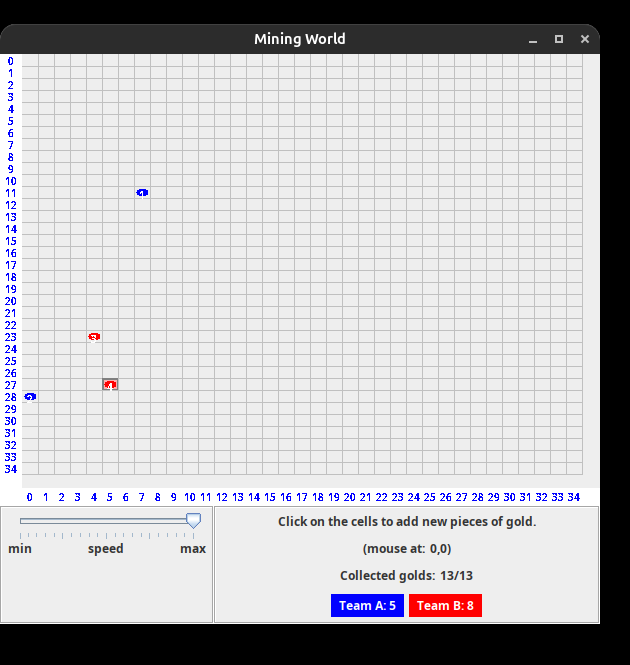
\includegraphics[width=0.6\textwidth]{imagens/battery_c4.png}
    \caption{Interface gráfica do ambiente Gold Miners após as alterações deste trabalho, com as duplas identificadas por cor, réguas de coordenadas e o placar por equipe no rodapé.}
    \label{fig:overview}
\end{figure}

\section{Descrição da solução desenvolvida}
\label{sec:solucao}

\subsection{Modelo de duplas}

O cenário base foi reorganizado em duas duplas, o Time A, formado por
miner1 e miner2, e o Time B, formado por miner3 e miner4. Os times são
definidos por crença (\texttt{team(miner1, teamA)}, e assim por diante) e o
ambiente passa a registrar o placar agregado por equipe
(\texttt{team\_score}), no lugar do placar individual do tutorial original.
Essa mudança é o que torna o cenário simultaneamente cooperativo, dentro da
dupla, e competitivo, entre duplas.

\subsection{Mecanismos de coordenação}

Cada mecanismo é implementado como uma crença ligável por agente no arquivo
de configuração do sistema multiagente (\texttt{use(...)}), o que permite testar cada
combinação de forma isolada.

\textbf{Reserva de tarefas (F1).} Um artefato compartilhado
(\texttt{GoldRegistry}) implementa a reserva exclusiva de uma peça de ouro.
Antes de perseguir um alvo, o minerador tenta reservá-lo no artefato, o que
impede que os dois integrantes da mesma dupla persigam ao mesmo tempo o
mesmo ouro. A reserva vale só entre os dois parceiros, as duas duplas
continuam disputando entre si pelo mesmo ouro.

\textbf{Capacidade e recrutamento (F2).} Cada minerador acompanha a
quantidade de ouro que já percebeu, mas ainda não foi tratada. Quando essa
quantidade passa de um limite definido, o agente pede ajuda ao parceiro. O
parceiro ocioso reage ao pedido e cruza o mapa para ajudar; caso o parceiro
também esteja ocupado, ele recusa o pedido, o que evita pedidos repetidos em
loop.

\textbf{Regiões estáticas (F3a).} O mapa é dividido ao meio pela coordenada
X, e cada integrante da dupla é responsável por uma metade. Ouro percebido
fora da própria região é repassado ao parceiro responsável por aquela
metade, por meio de comunicação direta.

\textbf{Proximidade dinâmica (F3b).} Os dois integrantes da dupla trocam
periodicamente a própria posição por comunicação direta. Ao perceber um novo
ouro, o agente compara a própria distância ao alvo com a distância do
parceiro, informada pela última posição recebida, e apenas o mais próximo
assume a tarefa.

\subsection{Correções no ambiente}

Durante o desenvolvimento, duas limitações do ambiente base foram
identificadas e corrigidas.

A primeira é a ausência de um critério de encerramento automático. No
tutorial original, os mineradores continuam vagando pelo mapa mesmo após
todo o ouro ser coletado. O ambiente foi alterado para registrar o fim da
simulação assim que todas as peças de ouro são entregues, com o placar final
e a identificação da equipe vencedora.

A segunda é uma célula de ouro inalcançável no canto do mapa. A rotina de
exploração sorteava a próxima posição a visitar usando
\texttt{jia.random(RX, W-1)}, que exclui o valor máximo do intervalo por
definição. Combinada à ação \texttt{go\_near}, que interrompe o deslocamento
assim que o agente fica vizinho do alvo, essa rotina nunca levava nenhum
agente a pisar na última linha ou coluna do mapa, e a percepção de vizinhança
3x3 nunca cobria a célula do canto (34, 34). O ouro nessa posição era, na
prática, impossível de ser descoberto. A correção substitui o sorteio por
\texttt{jia.random(RX, W)}, que passa a incluir o valor máximo do intervalo.

\section{Metodologia experimental}
\label{sec:metodologia}

A avaliação dos mecanismos de coordenação foi conduzida em duas frentes,
complementares entre si. A primeira é qualitativa, verifica se cada
mecanismo dispara o comportamento esperado a partir dos registros de
execução. A segunda é quantitativa, compara o placar por equipe do Time A,
sob diferentes combinações de mecanismos, ao placar do Time B, mantido
sempre ingênuo.

O experimento quantitativo usa o cenário de mapa 4 (grade 35x35, depósito na
posição (5, 27), treze peças de ouro, uma delas na posição de canto (34,
34)). O Time B não recebe nenhuma crença de coordenação em nenhuma
configuração, o que isola o efeito dos mecanismos do Time A sobre o
resultado. A \autoref{tab:configs} apresenta as cinco configurações
comparadas.

\begin{table}[H]
    \centering
    \caption{Configurações comparadas (C0 a C4).}
    \label{tab:configs}
    \begin{tabular}{lcccc}
        \hline
        \textbf{Configuração} & \textbf{Reserva (F1)} & \textbf{Regiões (F3a)} & \textbf{Proximidade (F3b)} & \textbf{Ajuda (F2)} \\
        \hline
        C0 -- Ingênuo               & Não & Não & Não & Não \\
        C1 -- Só reserva            & Sim & Não & Não & Não \\
        C2 -- Reserva + regiões     & Sim & Sim & Não & Sim \\
        C3 -- Reserva + proximidade & Sim & Não & Sim & Sim \\
        C4 -- Tudo                  & Sim & Sim & Sim & Sim \\
        \hline
    \end{tabular}
\end{table}

Cada configuração foi repetida cinco vezes, na velocidade máxima do
ambiente, sem atraso artificial entre ações, totalizando vinte e cinco
execuções. Um script de automação dispara cada execução, extrai o placar por
equipe a partir do registro de entregas no log e captura uma imagem da tela
na primeira repetição de cada configuração.

\section{Resultados}
\label{sec:resultados}

\subsection{Validação qualitativa dos mecanismos}

Os registros de execução confirmam que os quatro mecanismos disparam
conforme o comportamento projetado. A reserva de tarefas evita que os dois
integrantes de uma dupla persigam o mesmo ouro, e cada tentativa de reserva
é registrada no log antes da coleta. A capacidade e recrutamento aparece
quando um agente com ouro pendente acima do limite pede ajuda ao parceiro, que cruza
o mapa para ajudar quando está ocioso, e recusa o pedido quando também está
ocupado, sem gerar ciclos de repetição. As regiões estáticas e o roteamento
por proximidade também se comportam de acordo com a flag ativada,
redirecionando ouro fora da região do agente ou repassando o alvo ao
parceiro mais próximo.

O fim de jogo automático e a correção do ouro do canto (34, 34) foram
confirmados em execuções isoladas, com o log registrando a coleta das treze
peças de ouro e o encerramento da simulação com o placar final.

\subsection{Comparação quantitativa}

A \autoref{tab:resultados} apresenta a média de \texttt{team\_score} por
configuração, calculada sobre as cinco repetições de cada uma.

\begin{table}[H]
    \centering
    \caption{Média de \texttt{team\_score} por configuração (n = 5 repetições).}
    \label{tab:resultados}
    \begin{tabular}{lccc}
        \hline
        \textbf{Configuração} & \textbf{Time A (coordenado)} & \textbf{Time B (ingênuo)} & \textbf{Vencedor médio} \\
        \hline
        C0 & 5,2 & 6,8 & B \\
        C1 & 4,4 & 7,6 & B \\
        C2 & 4,2 & 7,6 & B \\
        C3 & 5,4 & 6,6 & B \\
        C4 & 4,4 & 7,6 & B \\
        \hline
    \end{tabular}
\end{table}

O Time B venceu, em média, em todas as configurações, inclusive em C0, na
qual nenhum dos dois times usa qualquer mecanismo de coordenação. O
resultado por configuração é ruidoso e sem um padrão claro em relação ao
número de mecanismos ativos, C3 (reserva, proximidade e ajuda) foi a única
configuração em que o Time A superou o baseline ingênuo C0, enquanto C1, C2
e C4 ficaram abaixo dele, mesmo C2 usando o mesmo número de mecanismos que
C3. Esse padrão se repete em relação a uma bateria anterior, executada sobre
o mesmo mapa, o que indica reprodutibilidade do efeito de o Time B vencer em
toda configuração, não ruído de uma única execução.

A \autoref{fig:battery} mostra o estado final de duas execuções da bateria,
a configuração C0, na qual nenhum mecanismo está ativo, e a configuração C4,
na qual todos os mecanismos do Time A estão ativos.

\begin{figure}[H]
    \centering
    \begin{subfigure}[b]{0.48\textwidth}
        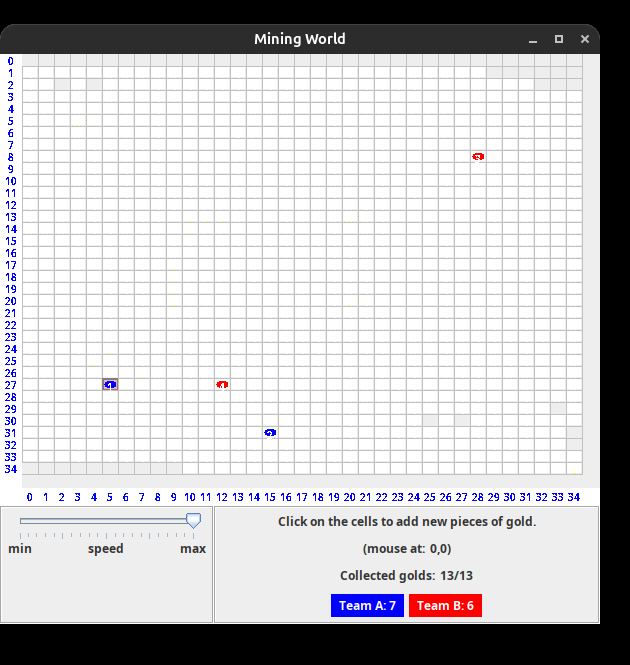
\includegraphics[width=\textwidth]{imagens/battery_c0.png}
        \caption{Configuração C0 (Time A ingênuo).}
    \end{subfigure}
    \hfill
    \begin{subfigure}[b]{0.48\textwidth}
        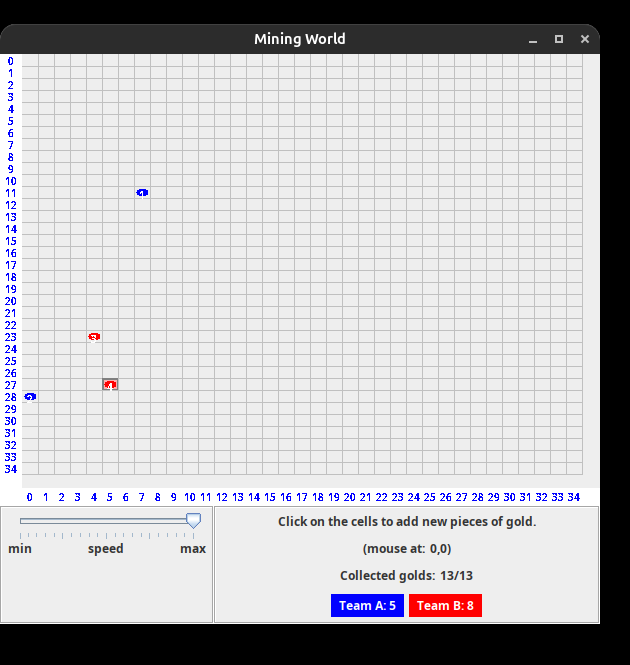
\includegraphics[width=\textwidth]{imagens/battery_c4.png}
        \caption{Configuração C4 (Time A com todos os mecanismos).}
    \end{subfigure}
    \caption{Estado final de execuções da bateria de comparação, primeira repetição de cada configuração.}
    \label{fig:battery}
\end{figure}

\subsection{Discussão}

A comparação quantitativa entre times não demonstra vantagem do time
coordenado sobre o ingênuo, resultado que não invalida a validação
qualitativa apresentada anteriormente, mas indica que o experimento de
comparação, do jeito que foi montado, não isola corretamente o efeito da
coordenação sobre o placar. Três fatores prováveis explicam esse resultado.

O primeiro, e mais relevante, é um viés de posição inicial. No mapa usado,
o segundo integrante do Time B nasce em uma posição que já corresponde a uma
célula de ouro, dentro de um agrupamento denso de sete peças. O Time A nasce
na borda superior do mapa, distante desse agrupamento. Como o Time B já
vence em C0, antes de qualquer coordenação entrar em jogo, essa vantagem de
posição inicial domina o resultado e mascara o efeito dos mecanismos
avaliados.

O segundo fator é o tamanho pequeno da amostra. Cinco repetições por
configuração produzem diferenças de poucas unidades entre médias, o que não
é suficiente para saber se o efeito é real ou só variação ao acaso.

O terceiro fator é que o mapa usado tem pouco ouro concentrado fora do
agrupamento citado. Isso reduz a disputa direta entre as duplas e, com ela,
as situações em que a coordenação, evitar colisão de alvo, redistribuir
carga, priorizar o agente mais próximo, faz diferença que apareça no
placar.

\subsection{Limitações}

Além do viés de posição inicial e do tamanho pequeno da amostra discutidos
na seção anterior, o experimento tem outras limitações que continuam
valendo mesmo se esses dois pontos forem corrigidos. A avaliação usa um
único mapa, o cenário 4, e não verifica se o padrão observado se repete em
mapas com outra distribuição de ouro ou com obstáculos. Das dezesseis
combinações possíveis entre os quatro mecanismos, apenas cinco foram
testadas, escolhidas para isolar o efeito de cada mecanismo individualmente,
o que deixa de fora combinações que poderiam mostrar uma interação diferente
entre eles. O experimento também compara sempre a mesma dupla ingênua fixa
contra a dupla coordenada, sem testar o efeito de cada mecanismo com as
posições iniciais das duas duplas trocadas.

\section{Conclusão}

Este trabalho estendeu o cenário Gold Miners para um modelo de duas duplas,
cooperativas internamente e competitivas entre si, e implementou quatro
mecanismos de coordenação entre os parceiros da dupla, a reserva de tarefas,
a capacidade e recrutamento entre parceiros, a divisão estática por regiões
e o roteamento dinâmico por proximidade. Os quatro mecanismos funcionam
conforme especificado, confirmado pelos registros de execução de cada
mecanismo isoladamente.

A comparação quantitativa entre o time coordenado e o time ingênuo, no
entanto, permanece inconclusiva, dominada por um viés de posição inicial
identificado no mapa usado, e não sustenta a conclusão de que a coordenação
melhora o placar nesse cenário específico. Esse resultado não invalida os
mecanismos implementados, mostra uma limitação de como o experimento foi
montado para avaliá-los.

Como sugestões para trabalhos futuros, destacam-se:

\begin{itemize}
    \item alternar as posições iniciais dos dois times entre execuções, de
    forma a cancelar o viés de posição identificado;
    \item usar um mapa com mais ouro concentrado, ambiente no qual a
    coordenação tem mais oportunidade de fazer diferença no placar;
    \item isolar cada execução da bateria em um processo Java próprio, para
    eliminar a leitura de registro residual entre execuções;
    \item aumentar o número de repetições por configuração, reportando média
    e desvio padrão.
\end{itemize}

Conclui-se que os mecanismos de coordenação propostos funcionam de acordo
com o comportamento projetado, e que uma avaliação quantitativa conclusiva
de seu efeito sobre o placar depende de corrigir o viés de posição inicial e
o isolamento de execução identificados neste relatório.

\subsection{Links utilizados}

O seguinte link do GitHub refere-se ao repositório onde os arquivos do
projeto podem ser encontrados:
\url{https://github.com/brenobmoreira/gold-miners}

\end{document}
